\chapter{Cosmological Solutions in Higher Dimensions}
\label{ch:brane}


To better understand the physical origin of the four-charge solution, we turn our attention to finding consistent higher-dimensional embeddings. This is motivated by the success of \cite{Dempster:2016}, which offered a new understanding of the Nernst solution \cite{Dempster:2015} by using a five-dimensional embedding. We are further motivated by the work of \cite{Cornalba:2003kd} and comments made by \cite{Burgess:2002vu} which link cosmological solutions to higher-dimensional theories reduced on orientifolds.

Before continuing, we remark on the work of \cite{Fre:2008zd}, in which a cosmological solution of the STU model was found. In this work, the authors also began by dimensionally reducing $\N = 2$ vector multiplet supergravity from four to three dimensions. Solutions are then derived through understanding the symmetric spaces associated to the sigma models. In contrast to our work, the authors explicitly search for cosmological rather than static solutions. The problem of uplifting the solution back to four dimensions becomes a problem in representation theory and their resulting four-dimensional spacetime has a general, but quite complicated form. The upshot is that the form of the line element derived has a coordinate structure which only yields a fragment of the solution that we found in Section \ref{sec:cosmologicalsolutionstu}. Specifically, their solution does not include the Killing horizon, and the static region and singularity are therefore not discussed. Their work has other virtues though, and several examples of cosmological solutions to $\N = 2$ supergravity are found. In particular, there is an interesting section in which they understand their solutions from a higher-dimensional perspective through a lift from four to ten dimensions on the orientifold $K3 \times T^2 / \mathbb{Z}_2$. The explicit relation between their solution and ours is complicated, and we will do not give the mapping. 

For our work, we will also study the cosmological solutions in ten and eleven dimensions, but instead of uplifting over the orientifold, we instead consider simpler, toroidal lifts. Despite this simplification, will are still able to relate our cosmological solution to black hole solutions of the STU model and to make contact with six-dimensional BPS solutions. By taking the extremal limit, we will be able to interpret our line elements as intersecting brane solutions from both a string and M-theory perspective.

We note here that in lifting of our solution over tori, we necessarily consider not the reduction of the full string theory, but some consistent truncation. This is because the reduction over the torus does not break any supersymmetry and so the naive reduction would produce $\N = 8$ supergravity in four dimensions. We also note that instead of reducing over an orientifold, we could also consider the decomposition of the fields while reducing over a Calabi-Yau threefold, which would break the right amount of supersymmetry, but do not comment on this further. 

This chapter is organised in the following way. First, we rewrite our Lagrangian \eq{4dlag} in a form that allows a direct comparison with \cite{Chow:2014cca}. We then uplift our non-extremal planar solutions of the STU model from four dimensions to five, six, ten and eleven dimensions, expressing our solutions as embedded into truncations of string/M-theory. Upon taking the extremal limit of the four-dimensional solution, we make contact with well-known brane configurations in string/M-theory models. Additional fine-tuning of the four-dimensional electric charges is shown to make the extremal six-dimensional uplift supersymmetric. This is a particularly surprising result as we did not utilise Killing spinor equations and therefore the existence of supersymmetric limit was not guaranteed.

\section{Dimensional lifting of the cosmological STU solution}
\label{sec:upliftstu}

In Section \ref{sec:studimred}, we performed the dimensional reduction of $\N = 1$, six-dimensional supergravity coupled to a tensor multiplet, recovering $\N = 2$ supergravity coupled to three vector multiplets in four dimensions. This is the STU model, for which we found planar symmetric solutions in Chapter \ref{ch:planarstu}. In this section, we reverse this procedure to obtain five and six-dimensional embeddings for the planar symmetric solutions. Furthermore, the five-dimensional solution can be uplifted over $T^6$ to give an eleven-dimensional line element, which is a solution of a consistent truncation of eleven-dimensional supergravity. Similarly, the six-dimensional solution can be uplifted over $T^4$, producing a ten-dimensional line element which is a solution to a consistent truncation of string theory.

We will follow the oxidation\footnote{The process of embedding lower-dimensional solutions in higher dimensions is sometimes called \emph{oxidation}, and has nothing to do with chemistry!} prescription of \cite{Chow:2014cca} to write down consistent truncated string/M-theory Lagrangians and their corresponding metric and gauge field content.

\subsection{Rewriting the Lagrangian for uplift}

Our starting point is the Lagrangian \eq{4dlag}, repeated here for reference
\begin{equation*}
 e_4^{-1} \La = -\frac{1}{2}R - g_{A\bar{B}} \partial_\mu z^A \partial^\mu \bar{z}^{\bar{B}} + \frac{1}{4} \I_{IJ} F^I_{\mu \nu} F^{J|\mu \nu} + \frac{1}{4} \cR_{IJ} F^I_{\mu \nu} \tilde{F}^{J|\mu \nu}.
\end{equation*}
To perform the uplift, we first find the exact form of the couplings in terms of our physical scalars $z^A$. The explicit expressions for the gauge couplings are obtained from the prepotential $F(X)$ using standard special geometry formulae. Full derivations for the couplings are given in appendix \ref{app:stucouplings}, in which we use the same conventions as \cite{Cortes:2009cs}.

Remembering that we have imposed the `purely imaginary' condition, the couplings take the form:
\begin{equation}
\label{eq:stucoup1}
 \cR_{IJ} = 0, \qquad  \I_{IJ} = \text{diag}\left( - s t u, -\frac{ t u}{s}, -\frac{s u}{t}, -\frac{ s t}{u} \right),
 \end{equation}
 \begin{equation}
 \label{eq:stucoup2}
 g_{A\bar{B}} = \text{diag}\left( \dfrac{1}{4s^2}, \dfrac{1}{4t^2}, \dfrac{1}{4u^2}\right),
\end{equation}
where
\begin{equation*}
 s = -\text{Im}(z^1) , \quad t = -\text{Im}(z^2), \quad u = -\text{Im}(z^3) .
\end{equation*}
When evaluating the couplings $\I_{IJ}$ on our solution, we find by inserting the value of the scalar fields \eq{stuphysicalscalars}
\begin{equation}
\label{eq:iij_coupling}	
    \I_{00}^2 = \frac{\Ham_0^3}{\Ham_1 \Ham_2 \Ham_3}, \qquad \I_{11}^2 = \frac{\Ham_0 \Ham_2 \Ham_3}{\Ham_1^3}, \qquad \I_{22}^2 = \frac{\Ham_0 \Ham_1 \Ham_3}{\Ham_2^3}, \qquad \I_{33}^2 = \frac{\Ham_0 \Ham_1 \Ham_2}{\Ham_3^3}.
\end{equation}
After redefining our scalars
\begin{equation}
 s = e^{-\phi_1}, \qquad t = e^{-\phi_2}, \qquad u = e^{-\phi_3},
\end{equation}
the Lagrangian takes the following form
\begin{equation}
\label{eq:stulag}
 \begin{aligned}
 e_4^{-1} \La = -\frac{1}{2}R - \frac{1}{4} \partial_\mu \phi_A \partial^\mu \phi_A
 - \frac{1}{4} e^{-\phi_1 - \phi_2 - \phi_3} \left[ (F^0)^2 + e^{2 \phi_A } (F^A)^2 \right] ,
 \end{aligned}
\end{equation}
\noindent where we sum over $A \in \{1,2,3\}$. Using the STU couplings (\ref{eq:stucoup1}) and the expressions for the physical scalrs \eq{stuphysicalscalars}, we can evaluate the scalars $\phi_i$ on our solution and thus express them
as functions of $\zeta$
\begin{equation*}
    e^{2\phi_1} = \frac{\I_{11}}{\I_{00}} = \frac{\Ham_2 \Ham_3}{\Ham_0 \Ham_1}
    , \quad e^{2\phi_2} = \frac{\I_{22}}{\I_{00}} = \frac{\Ham_1 \Ham_3}{\Ham_0 \Ham_2}
    , \quad e^{2\phi_3} = \frac{\I_{33}}{\I_{00}} =\frac{\Ham_1 \Ham_2}{\Ham_0 \Ham_3} \;.
\end{equation*}

To embed our solution into higher dimensions, we will use various ansatz given in \cite{Chow:2014cca} allowing for us to obtain the results for ten and eleven-dimensional solutions via six and five-dimensional solutions respectively. The relevant truncation of the four-dimensional STU Lagrangian given in \cite{Chow:2014cca} is
\begin{equation}
\label{eq:4dchow}
     e_4^{-1} \La_4 = -R - \frac{1}{2} \partial_\mu \varphi_i \partial^\mu \varphi_i
 - \frac{1}{4} e^{-\varphi_1 - \varphi_2 - \varphi_3} \left[ (\bF^4)^2 + e^{2 \varphi_i } (\tilde{\bF}_i)^2 \right] .
\end{equation}
This is related to our Lagrangian \eq{stulag} by an overall factor of 2, together with the following rescaling of the gauge fields and the scalars
\begin{equation*}
    F^0 = \frac{1}{\sqrt{2}} \bF^4, \qquad F^A = \frac{1}{\sqrt{2}} \tilde{\bF}_i, \qquad \phi_i = \varphi_i .
\end{equation*}
We will need to keep track of these factors while oxidising, and insert the exact values for the gauge fields into the ansatz of \cite{Chow:2014cca}.

\subsection{Oxidation to five dimensions}
The STU model can be consistently embedded into five dimensions with the bosonic Lagrangian
\begin{equation}
\label{eq:5dchow}
    \La_5 = - R \star 1 - \half h_i^{-2} \left(\star dh_i \wedge dh_i + \star \tilde{\bF}_i \wedge \tilde{\bF}_i \right) + \tilde{\bF}_1 \wedge \tilde{\bF}_2 \wedge \tilde{\mathbb{A}}_3,
\end{equation}
where the five-dimensional scalars $h^i$ satisfy the constraint $h_1 h_2 h_3 = 1$. Using the Kaluza-Klein reduction ansatz
\begin{equation}
\label{eq:5dan}
    ds_5 = f^{-1} ds_4^2 + f^2 (dz_5 - \mathbb{A}^4)^2 \;,\qquad \qquad \tilde{\mathbb{A}}_{(5D)i} = \tilde{\mathbb{A}}_i,
\end{equation}
we obtain the four-dimensional Lagrangian \eq{4dchow} when we make the choice $f h_i= e^{-\varphi_i}$. The vector field $\mathbb{A}^4$ is the Kaluza-Klein vector field, while the vector fields $\mathbb{A}_i$ descend from the five-dimensional vector fields.

Introducing new linear combinations $\sigma, \varphi, \lambda$ for the three independent real four-dimensional scalars by
\begin{equation*}
     \varphi_1 = -\frac{2}{\sqrt{6}} \sigma + \frac{1}{\sqrt{3}} \lambda, \quad \varphi_2 = -\frac{1}{\sqrt{2}} \phi + \frac{1}{\sqrt{6}} \sigma + \frac{1}{\sqrt{3}} \lambda, \quad \varphi_3 = \frac{1}{\sqrt{2}} \phi + \frac{1}{\sqrt{6}} \sigma + \frac{1}{\sqrt{3}} \lambda,
\end{equation*}
the five-dimensional constrained scalars $h^i$ can be expressed in terms of two independent fields
\begin{equation*}
 h_1 = e^{2 \sigma/\sqrt{6}}, \qquad h_2 = e^{\phi/\sqrt{2} - \sigma/\sqrt{6}}, \qquad h_3 = e^{-\phi/\sqrt{2} - \sigma/\sqrt{6}} \; .
\end{equation*}
Combining these two relations we obtain
\begin{equation*}
    \begin{aligned}
        h_1 &= \exp \left(-\frac{2\varphi_1}{3} + \frac{\varphi_2}{3} + \frac{\varphi_3}{3} \right) = \left( \frac{\I_{22} \I_{33} }{\I^2_{11}} \right)^{\frac{1}{6}}, \\
        h_2 &= \exp \left(\frac{\varphi_1}{3} - \frac{2\varphi_2}{3} + \frac{\varphi_3}{3} \right) = \left( \frac{\I_{11} \I_{33} }{\I^2_{22}} \right)^{\frac{1}{6}}, \\
        h_3 &= \exp \left(\frac{\varphi_1}{3} + \frac{\varphi_2}{3} - \frac{2 \varphi_3}{3} \right) = \left( \frac{\I_{11} \I_{22} }{\I^2_{33}} \right)^{\frac{1}{6}} ,
    \end{aligned}
\end{equation*}
and expressing the gauge couplings in terms of the harmonic functions $\Ham_i$,
\begin{equation}
\label{hi_Harmonic}
        h_i = \frac{\Ham_i}{(\Ham_1 \Ham_2 \Ham_3)^{\frac{1}{3}}} \; ,
\end{equation}
allows us to write down the Kaluza-Klein scalar $f$ in terms of $\zeta$
\begin{equation}
\label{eq:5dkk}
    f = e^{-\varphi_i} h_i^{-1} = \left(\frac{\I_{00}^3}{\I_{11} \I_{22} \I_{33}} \right)^{\frac{1}{6}}
    = \left( \frac{ \Ham_0^3}{\Ham_1 \Ham_2 \Ham_3} \right)^{1/6} \;.
\end{equation}
\subsection*{Five-dimensional metric}
Using \eq{5dan} together with \eq{5dkk} and $\mathbb{A}^4 = \sqrt{2} A^0$, as well as
collecting common factors, we obtain the following five-dimensional metric for the uplift of our four-charge solution:
\begin{equation}
\begin{aligned}
        ds^2_5 = (\Ham_1 \Ham_2 \Ham_3)^{-\frac{1}{3}} &\bigg[\Ham_0 dz_5^2 + \frac{\cW}{2\Ham_0}\left(\cW \frac{\gamma_0^2}{Q_0^2} + 1 \right) d\eta^2 - \frac{\cW \gamma_0}{\sqrt{2} Q_0} d\eta dz_5 \\ &+ 2\Ham_1 \Ham_2 \Ham_3 \left(- \frac{ d\zeta^2}{\cW} + dx^2 + dy^2 \right) \bigg].
\end{aligned}
\end{equation}

\subsection*{Five-dimensional gauge potential}

To obtain expressions for the five-dimensional gauge potentials,
it is necessary to express all the gauge fields in our solution in terms of electric components. This
requires replacing the dual vector potentials $\tilde{A}_A$ by the `standard'
 vector potentials $A^A$. The associated field strength $\tilde{F}_A$ and $F^A$ are related by Hodge duality together with multiplication by inverse gauge coupling matrix
 \begin{equation*}
    F^A = -\I^{AB} \star \tilde{F}_B.
\end{equation*}
Using the form of the gauge potential found in \eq{new4dgauge}, standard calculations give their form
\begin{equation}
\label{eq:5dfield}
    F^A = -\I^{AB} \star \tilde{F}_B = - \frac{P^A}{2\sqrt{\gamma_0 \gamma_1 \gamma_2 \gamma_3}} dx \wedge dy.
\end{equation}
Integrating and relating to the gauge fields in our ansatz, we obtain the form of the three five-dimensional vector potentials
\begin{equation}
\label{eq:5dvec}
    \tilde{\mathbb{A}}_i = \sqrt{2} A^A = \mathfrak{p}_a \left(y dx - x dy \right), \qquad \mathfrak{p}_a = \frac{ P^a}{2 \sqrt{2 \gamma_0 \gamma_1 \gamma_2 \gamma_3}} .
\end{equation}
We will return to these gauge fields before uplifting the solution to six dimensions, when it will be necessary to Hodge dualise in five dimensions to obtain a two-form potential.

\subsection*{Extremal limit}
We now investigate the effect of the four-dimensional extremal limit defined in Section \ref{sec:4Dext} for the following higher-dimensional lifts.\footnote{We note here that we use the same symbols $h_a$ for the integration constants in \eq{extlim} and the constrained five-dimensional scalars, as this allows us to match notation with the literature on five-dimensional solutions. We trust that the reader will infer from context which quantity is meant in a particular expression.} Just as in the four-dimensional case, the horizon for the five-dimensional solution is pushed out to $\zeta \rightarrow \infty$ and the static region takes up the entirety of our spacetime; in other words, the extremal limit results in a solution containing a naked singularity. Simplifying the metric functions using the expressions from \eq{extlim} we can write down the five-dimensional line element in the form
\begin{equation*}
    ds^2_5 = (\Ham_1\Ham_2\Ham_3)^{-\frac{1}{3}} \left[d\eta dz_5 + \Ham_0 dz_5^2 + \Ham_1\Ham_2\Ham_3 (d\zeta^2 + dx^2 + dy^2) \right].
\end{equation*}
We will consider the extremal limit for each of the following uplifts as we further oxidise the STU model.

\subsection{Oxidation to eleven dimensions}
To uplift our solution to eleven dimensions, we start with the bosonic part of the eleven-dimensional supergravity Lagrangian
\begin{equation*}
    \La_{11} = -R \star 1 - \half \star \mathcal{F} \wedge \mathcal{F} - \frac{1}{6} \mathcal{F} \wedge \mathcal{F} \wedge \mathcal{A},
\end{equation*}
where $\mathcal{A}$ is the three-form such that $\mathcal{F} =d\mathcal{A}$ is the four-form field strength. We can directly embed the five-dimensional STU model into this theory through a Kaluza-Klein reduction on $T^6$ with the ansatz
\begin{equation*}
    ds_{11}^2 = ds_5^2 + h_1 (dy_1^2 + dy_2^2) + h_2 (dy_3^2 + dy_4^2) + h_3 (dy_5^2 + dy_6^2),
\end{equation*}
\begin{equation*}
    \mathcal{A} = \tilde{\mathbb{A}}_1 \wedge dy^1 \wedge dy^2 + \tilde{\mathbb{A}}_2 \wedge dy^3 \wedge dy^4 + \tilde{\mathbb{A}}_3 \wedge dy^5 \wedge dy^6.
\end{equation*}
In a consistent truncation to five-dimensional minimal supergravity, the volume of the torus corresponds to a scalar in a hypermultiplet, while its shape is encoded by scalars in vector multiplets. This factorisation imposes the condition $h_1 h_2 h_3=1$ on the scalars $h_i$. By restricting our field content, we can consistently truncate out the hypermultiplets and remain with the five-dimensional STU model with two vector multiplets.

We now combine this $5D/11D$ lift with the previous $4D/5D$ lift. In our four-dimensional solution, we can express the $h_i$ as functions of $\zeta$ through the harmonic functions $\Ham_i$, see (\ref{hi_Harmonic}). The three-form gauge potential is found directly from the components of \eq{5dvec}. Thus the full line element for the eleven-dimensional lift of the non-extremal planar solution to the four-dimensional STU model is
\begin{equation}
\label{eq:11Dmet}
\begin{aligned}
        ds^2_{11} = (\Ham_1 \Ham_2 \Ham_3)^{-\frac{1}{3}} &\bigg[\Ham_0 dz_5^2 + \frac{\cW}{2\Ham_0}\left(\cW \frac{\gamma_0^2}{Q_0^2} + 1 \right) d\eta^2 - \frac{\cW \gamma_0}{\sqrt{2} Q_0} d\eta dz_5 \\ &+ 2\Ham_1 \Ham_2 \Ham_3 \left(- \frac{ d\zeta^2}{\cW} + dx^2 + dy^2 \right) \\
        &+ \Ham_1 (dy_1^2 + dy_2^2) + \Ham_2 (dy_3^2 + dy_4^2) + \Ham_3 (dy_5^2 + dy_6^2)
        \bigg] \;.
\end{aligned}
\end{equation}

\subsection*{Eleven-dimensional extremal limit}
By again substituting in the four-dimensional extremal limit \eq{extlim} we can write down \eq{11Dmet} in the extremal limit to find
\begin{equation}
\begin{aligned}
\label{eq:11dstuextremal}
    ds_{11}^2 = &(\Ham_1\Ham_2\Ham_3)^{-\frac{1}{3}} \big[ d\eta dz_5 + \Ham_0 dz_5^2 + \Ham_1\Ham_2\Ham_3 (d\zeta^2 + dx^2 + dy^2) \\
    &+ \Ham_1(dy_1^2 + dy_2^2) + \Ham_2(dy_3^2 + dy_4^2) + \Ham_3(dy_5^2 + dy_6^2) \big].
\end{aligned}
\end{equation}
This extremal solution should remind the reader of the line element \eq{triplem5wave} introduced in Section \ref{sec:intersecting} which described the configuration of three M5 branes intersecting over a string, encoded by $\Ham_1, \Ham_2,\Ham_3$, with a PP-wave superimposed along the intersection direction, encoded by $\Ham_0$ \cite{Tseytlin:1996bh}. For solutions with spherical symmetry, which in Section \ref{sec:intersecting} is enforced by the harmonic functions encoded by $H_i$, compactification on $T^6 \times S^1$ gave rise to four-charged, BPS black holes. For these solutions, the branes are delocalised along $y^1, \ldots, y^6$ but localised in the remaining three spacelike directions. The four-dimensional line element is given in \eq{triplem5red} and a deeper discussion for these solutions and their relationship to $\N = 2$ supergravity appears in \cite{Behrndt:1996jn}. There is a crucial difference between those solutions and our extremal configuration \eq{11dstuextremal}, which can be seen in the harmonic functions $\Ham_a$. In our solutions, the M5 branes have in addition been further delocalised in two of the non-compact directions, which upon the reduction over $T^6 \times S^1$, will give rise to planar rather than spherical symmetry which was imposed at the level of the metric ansatz. 

\subsection{Oxidation to six dimensions}

Lifting the four-dimensional Lagrangian to six dimensions by extending the $4D/5D$ lift requires a tweak of the five-dimensional Lagrangian, namely to Hodge-dualise one of the three vector potentials into a two-form $B$. This is the reverse process of the computation we performed in Section \ref{sec:studimred}, where we dualise the three-form so we can reduce all three 2-form field strengths in the same way. The reason we dualise before uplifting is that the six-dimensional supergravity is chiral and both the supergravity multiplet and tensor multiplets contain self-dual or anti-self-dual tensor fields which do not admit a standard Lagrangian description. However, in supergravity coupled to one tensor multiplet (plus vector and hypermultiplets), one self-dual and one anti-self-dual tensor combine into an unconstrained tensor, which allows a standard Lagrangian description. String compactifications to six dimensions are of this type, with the tensor field descending from the ten-dimensional Kalb-Ramond field.

Matching our conventions with the work of \cite{Chow:2014cca} we define the three-form from the dualisation of the two-form field strength in five dimensions
\begin{equation}
\label{eq:hodtra}
    \tilde{\bF}_3 = d\tilde{\mathbb{A}}_3 = -h_1^{-2} h_2^{-2} \star_5 \mathbb{H} .
\end{equation}
Making this transformation and substituting into the Lagrangian results in
\begin{equation}
\begin{aligned}
        \label{eq:5dchow2}
    \La_5 = &- R \star 1 - \half h_i^{-2} \star dh_i \wedge dh_i +\half h_1^{-2} \star \tilde{\bF}_1 \wedge \tilde{\bF}_1 \\
    &+ \half h_2^{-2} \star \tilde{\bF}_2 \wedge \tilde{\bF}_2 - \half h_1^{-2} h_2^{-2} \star \mathbb{H} \wedge \mathbb{H} .
\end{aligned}
\end{equation}
We can now use the results of \cite{Chow:2014cca}, and first work with the new three-form field strength in five dimensions in terms of $\zeta$.

\subsection*{Dualisation of the five-dimensional gauge field}
Taking the Hodge dual of \eq{hodtra} we find the three-form
\begin{equation*}
        \star_5 \mathbb{H} = - h^2_1 h^2_2 \tilde{\bF}_3 \;,\qquad
        \star_5 \star_5 \mathbb{H} = - \star_5(h^2_1 h^2_2 \tilde{\bF}_3) \;, \qquad
        \mathbb{H} = \star_5(h^2_1 h^2_2 \tilde{\bF}_3) \;,
\end{equation*}
where we have used that for a $k$-form $\omega$ in $n$ dimensions in the Lorentzian signature $\star \star \omega = (-1)^{k(n-k)+1} \omega$. Substituting in \eq{5dfield} together with:
\begin{equation*}
    \sqrt{-g_5} = 2 (\Ham_1 \Ham_2 \Ham_3)^{\frac{2}{3}}
, \qquad \epsilon_{\eta \zeta x y z_5} = 1 \;,
\end{equation*}
\begin{equation*}
    h_1^2 h_2^2 = h_3^{-2} = (\Ham_1 \Ham_2)^{\frac{2}{3}} \Ham_3^{-\frac{4}{3}}, \qquad g^{xx} = g^{yy} = \half(\Ham_1 \Ham_2 \Ham_3)^{-\frac{2}{3}},
\end{equation*}
we find that the three-form is
\begin{equation*}
        \mathbb{H} = -\left( \frac{ \mathfrak{p}_3}{\Ham_3^2} \right) d\eta \wedge d\zeta \wedge dz_5 \;.
\end{equation*}

\subsection*{Lift to six dimensions}

The six-dimensional Lagrangian is
\begin{equation*}
    \La_6 = - R\star 1 - \half \star d\phi \wedge d\phi - \half e^{-\sqrt{2}\phi} \star H \wedge H,
\end{equation*}
where $H = dB$ is a three-form field strength. The reduction ansatz which
reproduces our five-dimensional Lagrangian (\ref{eq:5dchow2}) is
\begin{equation*}
    ds^2_6 = e^{\sigma/\sqrt{6}} ds_5^2 + e^{-3\sigma/\sqrt{6}} (dz_6 + \tilde{\mathbb{A}}_1)^2 \;,\qquad B_{(6D)} = B + \tilde{\mathbb{A}}_2 \wedge (dz_6 + \tilde{\mathbb{A}}_1),
\end{equation*}
with the field strengths decomposed as
\begin{equation*}
H_{(6D)} = \mathbb{H} + \tilde{\bF}_2 \wedge (dz_6 + \tilde{\mathbb{A}}_1) \;,    \qquad \mathbb{H} = dB - \tilde{\mathbb{A}}_2 \wedge \tilde{\bF}_1 ,\qquad \tilde{\bF}_i = d \tilde{\mathbb{A}}_i \;.
\end{equation*}
We see that from our parameterisation of the $h_i$ we can write the six-dimensional Kaluza-Klein scalar as
\begin{equation*}
    e^{\sigma/\sqrt{6}} = \sqrt{h_1} = \left( \frac{\Ham_1^3}{\Ham_1 \Ham_2 \Ham_3} \right)^{\frac{1}{6}} \;.
\end{equation*}

We are now in the position to combine these results to write down the six-dimensional metric for our embedded solution:
\begin{equation*}
\begin{aligned}
        ds^2_6 = (\Ham_2 \Ham_3)^{-\frac{1}{2}} &\bigg[\Ham_0 dz_5^2 + \frac{\cW}{2\Ham_0}\left(\cW \frac{\gamma_0^2}{Q_0^2} + 1 \right) d\eta^2 - \frac{\cW \gamma_0}{\sqrt{2} Q_0} d\eta dz_5 \\ &+ 2\Ham_1 \Ham_2 \Ham_3 \left(- \frac{ d\zeta^2}{\cW} + dx^2 + dy^2 \right) \bigg] + \frac{(\Ham_2 \Ham_3)^\half}{\Ham_1} (dz_6 + \tilde{\mathbb{A}}_1)^2 \;,
\end{aligned}
\end{equation*}
where the determinant of the metric is
\begin{equation*}
    \sqrt{-g_6} = 2 \Ham_1 \sqrt{\Ham_2 \Ham_3} \;.
\end{equation*}
The piece containing the gauge field $\mathbb{A}_1$ can be expanded
\begin{equation*}
\begin{aligned}
        (dz_6 + \tilde{\mathbb{A}}_1)^2 &= (dz_6 + (\tilde{\mathbb{A}}_1)_x dx + (\tilde{\mathbb{A}}_1)_y dy)^2 \;,\\
        &= (dz_6 + \mathfrak{p}_1(ydx - xdy))^2 \;.
\end{aligned}
\end{equation*}


\subsection*{Six-dimensional gauge fields}
We now take the gauge fields and express them as a function of the six-dimensional coordinates. We see that for the two remaining one-form potentials, nothing has been changed compared to the lower-dimensional solutions:
\begin{equation*}
    \tilde{\mathbb{A}}_1 = \sqrt{2} A^1, \qquad \tilde{\mathbb{A}}_2 = \sqrt{2} A^2 \;.
\end{equation*}
The three-form $H$ is found from two pieces
\begin{equation*}
    H_{(6D)} = \mathbb{H} + \tilde{\mathbb{F}}_2 \wedge ( dz_6 + \tilde{\mathbb{A}}_1) \;.
\end{equation*}
This is simplified, as the term
\begin{equation*}
    \tilde{\mathbb{F}}_2 \wedge \tilde{\mathbb{A}}_1 = 2 \mathfrak{p}_2 dx \wedge dy \wedge \mathfrak{p}_1 \left(y dx - xdy \right) = 0,
\end{equation*}
is zero due to anti-symmetry. Using the work from the five-dimensional calculations, the six-dimensional three-form field strength is given by:
\begin{equation*}
\begin{aligned}
        H_{(6D)} = -\left( \frac{ \mathfrak{p}_3}{\Ham_3^2} \right) d\eta \wedge d\zeta \wedge dz_5
 -( 2\mathfrak{p}_2) dx \wedge dy \wedge dz_6 \;.
\end{aligned}
\end{equation*}


\subsection*{Six-dimensional extremal limit}
Taking the extremal limit \eq{extlim}, the six-dimensional line element is given by
\begin{equation}
\label{eq:6dmet}
    ds_6^2 = \sqrt{\frac{\Ham_2}{\Ham_3}} \left[\Ham_2^{-1} \left(\Ham_0 dz_5^2 + dz_5d\eta \right) + \Ham_3 \Ham_1 (d\zeta^2 + dx^2 + dy^2) + \Ham_3 \Ham_1^{-1}(dz_6 +\tilde{\mathbb{A}}^1)^2 \right].
\end{equation}
The three-form in this limit is given by
\begin{equation*}
        H_{(6D)} = -\left( \frac{ \mathfrak{p}_3}{\Ham_3^2} \right) d\eta \wedge d\zeta \wedge dz_5
 -( 2\mathfrak{p}_2) dx \wedge dy \wedge dz_6, \qquad \mathfrak{p}_a = \frac{ P^a}{2 \sqrt{2 Q_0 P^1 P^2 P^3}}.
\end{equation*}


\subsection{Oxidation to ten dimensions}
\label{sec:to10d}
The six-dimensional STU model is a consistent truncation of the reduction of type IIB supergravity compactified over $T^4$. To lift our solution, we only need to include the overall volume of the $T^4$ as a modulus
\begin{equation*}
    ds_{10}^2 = ds_6^2 + e^{\phi / \sqrt{2} }(dy_1^2 + dy_2^2 + dy_3^2 + dy_4^2), \qquad \Phi = \frac{\phi}{\sqrt{2}}, \qquad C \equiv B.
\end{equation*}
The expression for the six-dimensional dilaton $\phi$ in terms of $\zeta$ is
\begin{equation*}
    e^{\sqrt{2} \phi} = \frac{h_2}{h_3} = \left(\frac{\I_{33} }{\I_{22}}\right)^{\frac{1}{2}} \quad \Rightarrow \quad e^{\phi / \sqrt{2} } = \left(\frac{\I_{33} }{\I_{22}}\right)^{\frac{1}{4}} = \sqrt{\frac{\Ham_2}{\Ham_3}} \;.
\end{equation*}
All other data follow straight from the six-dimensional solutions.
The ten-dimensional dilaton is given by
\begin{equation*}
    \Phi = \half \log \left(\frac{\Ham_2}{\Ham_3} \right).
\end{equation*}
The ten-dimensional line element is given by
\begin{equation*}
\begin{aligned}
        ds^2_{10} = \sqrt{\frac{\Ham_2}{\Ham_3}} &\bigg[\Ham_0 \Ham_2^{-1} dz_5^2 + \frac{\cW}{2\Ham_0 \Ham_2}\left(\cW \frac{\gamma_0^2}{Q_0^2} + 1 \right) d\eta^2 - \frac{\cW \gamma_0}{\sqrt{2} Q_0 \Ham_2} d\eta dz_5 \\ &+ 2\Ham_1 \Ham_3 \left(- \frac{ d\zeta^2}{\cW} + dx^2 + dy^2 \right) + \frac{\Ham_3}{\Ham_1} (dz_6 + \tilde{\mathbb{A}}_1)^2 \\
        &+ dy_1^2 + dy_2^2 + dy_3^2 + dy_4^2 \bigg].
\end{aligned}
\end{equation*}

\subsection*{Ten-dimensional extremal limit}
Uplifting the extremal six-dimensional solution using the same methods as Section (\ref{sec:to10d}) we find that the line element is
\begin{equation}
\label{eq:10extremald1d5}
\begin{aligned}
        ds^2_{10} = &\sqrt{\frac{\Ham_2}{\Ham_3}} \bigg[\Ham_2^{-1} \left(\Ham_0 dz_5^2 + dz_5d\eta \right) + \Ham_3 \Ham_1 (d\zeta^2 + dx^2 + dy^2) \\ &+ \Ham_3 \Ham_1^{-1}(dz_6^2 + \tilde{\mathbb{A}}^1)^2 + dy_1^2 + dy_2^2 + dy_3^2 + dy_4^2\bigg].
\end{aligned}
\end{equation}
As with the eleven-dimensional uplift, we can recognise this line element as a solution for an intersecting brane configuration. We can compare this with the line element \eq{d1d5kkpp}, which is the solution for the D1-D5 brane intersection with a PP-wave superimposed over the intersection direction, and a Taub-NUT space in the relative transverse space. In Section \ref{sec:intersecting}, we showed that upon reduction over a $T^6$, the solution \eq{d1d5kkppred} gave rise to a four-dimensional black hole solution with a finite area, which interpolated between an $AdS_2 \times S^2$ on the horizon to Minkowski at asymptotic infinity. Here, in the solution \eq{10extremald1d5} the key difference is again the linear harmonic functions. Where as before the zeros of $H_i$ signalled the location of the brane, the planar symmetry imposed in four dimensions leads to linear harmonic functions $\Ham_a$, and we understand the brane configuration \eq{10extremald1d5} as being smeared over two additional dimensions.


\section{Supersymmetry in six dimensions}
\label{sec:susy6d}

Supersymmetric solutions of six-dimensional supergravity have been classified in detail. The first classification of supersymmetric solutions in the minimal ungauged six-dimensional theory, with a self-dual three-form, was constructed in \cite{Gutowski:2003rg}. Following on from this, the supersymmetric solutions of six-dimensional U(1), and SU(2) gauged supergravity were classified in \cite{Cariglia:2004kk}. This analysis was done using the spinor bilinears method. Supersymmetric solutions of more general theories coupled to arbitrary vector and tensor multiplets were classified using spinorial geometry methods in \cite{Akyol:2010iz}; see also \cite{Akyol:2012cq, Akyol:2013ana, Cano:2018wnq, Lam:2018jln}. These classifications have been used to find many new examples of solutions, and we shall show that in a certain limit, the six-dimensional solution we have constructed satisfies the necessary and sufficient conditions for supersymmetry.

\subsection{Conditions required for supersymmetry}

We now turn our attention to the six-dimensional uplift of our solution and test to see whether there is a configuration of integration constants such that the solution is supersymmetric. In this particular case, the theory of interest is the $U(1)$ gauged supergravity whose supersymmetric solutions were classified in \cite{Cariglia:2004kk}, in the special case for which the $U(1)$ gauge parameter is set to zero. The bosonic content of this theory is the metric $g$, a real three-form $G$, and a dilaton $\phi$. The geometry of these solutions was also considered in \cite{Bena:2011dd}. Before considering the six-dimensional uplift in detail, we first summarise the necessary and sufficient conditions on the bosonic fields in order for a generic solution of this theory to be supersymmetric.

The metric for the supersymmetic solutions is given by
\begin{equation}
\label{eq:benamet}
    ds^2_6 = -2H^{-1} (dv + \beta) (du + \omega + \half \mathcal{F}(dv+\beta)) + H ds_4^2.
\end{equation}
The metric for the four-dimensional base space $\mathcal{B}$ is written as
\begin{equation}
    ds^2_4 = h_{mn}dx^m dx^n,
\end{equation}
with $\mathcal{F}$ and $H$ as smooth functions and $\beta=\beta_m dx^m$ and $\omega = \omega_m dx^m$ regarded as one-forms on $\mathcal{B}$. The vector ${\partial \over \partial u}$ corresponds to a Killing spinor bilinear and the Killing spinor equations imply that this vector is an isometry, and moreover, that the Lie derivative of the three-form $G$ and the dilaton $\Phi$ with respect to ${\partial \over \partial u}$ vanish. However, in general, the metric, the three-form and the dilaton may depend on the $v$ and the $x^m$ coordinates.


Analysis of the algebraic properties of the spinor bilinears through considering the Fierz identities implies that there are three anti-self-dual two-forms on the base ${\cal{B}}$: $J^{(A)}$, $A=1,2,3$, which
satisfy the algebra of the imaginary unit quaternions; ${\cal{B}}$ therefore admits an almost hyper-K\"ahler structure. In addition, the
gravitino Killing spinor equations imply that
\begin{eqnarray}
\label{almosthk}
{\tilde{d}} J^{(A)} = \partial_v \bigg( \beta \wedge J^{(A)} \bigg) \; ,
\end{eqnarray}
where ${\tilde{d}}$ denotes the exterior derivative restricted to surfaces of constant $u$ and $v$;
and $\partial_v$ denotes the Lie derivative with respect to ${\partial \over \partial v}$.
It is also useful to define the differential operator $D$ by
\begin{eqnarray}
D \chi = {\tilde{d}} \chi - \beta \wedge \partial_v \chi,
\end{eqnarray}
where $\chi$ is a $u$-independent differential form on ${\cal{B}}$.
Then supersymmetry implies that
\begin{eqnarray}
D \beta = \star_4 D \beta,
\end{eqnarray}
where $\star_4$ denotes the Hodge dual on ${\cal{B}}$. This exhausts the conditions on the
geometry obtained from the gravitino Killing spinor equation. It remains to consider
the conditions on the fluxes.

The Killing spinor equations determine the components of the three-form $G$ as
\begin{equation}
\begin{aligned}
    e^{\sqrt{2} \Phi } G &= \tfrac{1}{2} \star_4 \left(DH + H \partial_v \beta - \sqrt{2} H D \Phi \right) \\
    &- \tfrac{1}{2} e^+ \wedge e^- \wedge \left(H^{-1} DH + \partial_v \beta + \sqrt{2} D \Phi \right) \\
    &- e^+ \wedge (-H \psi + \tfrac{1}{2} (D\omega)^- -K) + \tfrac{1}{2} H^{-1} e^-\wedge D \beta,
\end{aligned}
\label{susythree}
\end{equation}
where $K$ is a self-dual form on the base ${\cal{B}}$, $\psi$ is expressed as
\begin{eqnarray}
\psi = {1 \over 16} H \epsilon_{ABC} J^{(A) mn} (\partial_v J^{(B)})_{mn} J^{(C)},
\label{psidef}
\end{eqnarray}
and we have adopted the null basis
\begin{eqnarray}
e^+ = H^{-1} \big(dv+\beta), \qquad e^-= du+\omega +{1 \over 2} {\cal{F}} H e^+, \qquad
e^a= H^{1 \over 2} {\tilde{e}}^a,
\end{eqnarray}
in which the metric is
\begin{eqnarray}
ds^2_6 =-2 e^+ e^- + \delta_{ab} e^a e^b,
\end{eqnarray}
and the basis ${\tilde{e}}^a= {\tilde{e}}^a{}_m dx^m$ is a basis for the base ${\cal{B}}$.

On imposing the Bianchi identity $dG = 0$, the following conditions are obtained
\begin{eqnarray}
\label{bian61}
D \bigg(H^{-1} e^{\sqrt{2} \Phi} \big(K-H {\cal{G}}-H \psi \big) \bigg)
+{1 \over 2}\partial_v \star_4 \bigg(D \big(H e^{\sqrt{2} \Phi}\big)+H e^{\sqrt{2}\Phi} \partial_v \beta \bigg)
\nonumber \\
-H^{-1} e^{\sqrt{2} \Phi} (\partial_v \beta) \wedge \big(K-H {\cal{G}}-H \psi \big)=0,
\end{eqnarray}
and
\begin{eqnarray}
\label{bian62}
-D \bigg(H^{-1} e^{-\sqrt{2} \Phi} \big(K+H {\cal{G}}+H \psi \big) \bigg)
+{1 \over 2}\partial_v \star_4 \bigg(D \big(H e^{-\sqrt{2} \Phi}\big)+H e^{-\sqrt{2}\Phi} \partial_v \beta \bigg)
\nonumber \\
+H^{-1} e^{-\sqrt{2} \Phi} (\partial_v \beta) \wedge \big(K+H {\cal{G}}+H \psi \big)=0,
\nonumber \\
\end{eqnarray}
where
\begin{eqnarray}
{\cal{G}}= {1 \over 2H} \bigg( \big(D \omega\big)^+ +{1 \over 2}{\cal{F}} D \beta \bigg),
\end{eqnarray}
and $(D \omega)^\pm$ denote the self-dual and anti-self dual parts of $D \omega$.

The gauge field equations, $d (e^{2 \sqrt{2} \Phi} \star_6 G)=0$ also imply the following conditions
\begin{eqnarray}
\label{gauge61}
D \star_4 \bigg(D \big(H e^{\sqrt{2} \Phi} \big) + H e^{\sqrt{2} \Phi} \partial_v \beta \bigg)
= 2 H^{-1} e^{\sqrt{2} \Phi} \big(K-H {\cal{G}} \big) \wedge D \beta,
\end{eqnarray}
and
\begin{eqnarray}
\label{gauge62}
D \star_4 \bigg(D \big(H e^{-\sqrt{2} \Phi} \big) + H e^{-\sqrt{2} \Phi} \partial_v \beta \bigg)
= -2 H^{-1} e^{-\sqrt{2} \Phi} \big(K+H {\cal{G}} \big) \wedge D \beta.
\end{eqnarray}

As noted in \cite{Cariglia:2004kk}, imposing these conditions implies that the dilaton field equation is automatically satisfied, and also all but one component of the Einstein field equations also hold. The remaining $++$ component of the Einstein equations must be imposed
as an additional condition. On defining
\begin{eqnarray}
L=\partial_v \omega +{1 \over 2} {\cal{F}} \partial_v \beta -{1 \over 2}D {\cal{F}},
\end{eqnarray}
this component of the Einstein equation is given by
\begin{eqnarray}
\star_4 D \star_4 L &=&{1 \over 2} h^{mn} \partial_v^2 \big(H h_{mn} \big)
+{1 \over 2} \partial_v \big(H h^{mn} \big) \partial_v \big(H h_{mn} \big)\nonumber \\
&-& {1 \over 2} H^{-2} \big(D \omega +{1 \over 2} {\cal{F}} D \beta \big)^2 -2 L^m ({\partial_v} \beta)_m+2 H^2 (\partial_v \Phi)^2
\nonumber \\
&+& 2 H^{-2} \big(K-H \psi +{1 \over 2} (D \omega)^- \big)^2.
\label{nulleinst}
\end{eqnarray}
where we adopt the convention that if $X$ is a two-form on ${\cal{B}}$ then $X^2={1 \over 2} X_{mn} X^{mn}$.


\subsection{Matching the solutions}

We now wish to see whether we can satisfy the conditions outlined above for the extremal solution \eq{6dmet}. We begin by taking the $\alpha \rightarrow 0$ limit; in four dimensions we can think of this limit as taking the blackening factor to zero and thus, being associated with extremality. In this limit, the resulting metric was found to be \eq{6dmet} and for convenience, we repeat the full expression for the six-dimensional three-form
\begin{equation}
\begin{aligned}
        H_{(6D)} = -\frac{P^3}{2\Ham_3^2 \sqrt{2 Q_0 P^1 P^2 P^3}} d\eta \wedge d\zeta \wedge dz_5 - \frac{P^2}{\sqrt{2 Q_0 P^1 P^2 P^3}} dx \wedge dy \wedge dz_6.
\end{aligned}
\label{threeform6}
\end{equation}
Comparing our metric with the metric \eq{benamet} we extract a four-dimensional base space:
\begin{equation}
    ds^2_6 = (\Ham_2 \Ham_3)^{-\half} dz_5 (d\eta + \Ham_0 dz_5) + (\Ham_2 \Ham_3)^{\half} ds_4^2 ,
\end{equation}
in the form
\begin{equation}
\label{eq:4dbase}
    ds^2_4 = \Ham_1 ( d\zeta^2 + dx^2 + dy^2) + \Ham_1^{-1} (dz_6 + \mathbb{A}^1)^2 .
\end{equation}
Direct comparison to \eq{benamet} shows that we should make the following identifications:
\begin{equation*}
 \beta = \omega = 0, \qquad H = \sqrt{\Ham_2 \Ham_3}, \qquad \mathcal{F} = \Ham_0, \qquad dv = dz_5, \qquad 2du = d\eta    ,
\end{equation*}
with all components of the metric and three-form independent of the $v$ coordinate. The basis vectors are given as:
\begin{equation*}
    \begin{aligned}
        e^+ = (\Ham_2 \Ham_3)^{-\half} dz_5, \qquad e^- = \half d\eta + \half \Ham_0 dz_5, \qquad e^a = (\Ham_1 \Ham_2)^{\frac{1}{4}}\tilde{e}^a_m dx^m .
    \end{aligned}
\end{equation*}


We begin by looking more closely at the base space
\eq{4dbase}
\begin{equation*}
    ds^2_4 = \Ham_1 ( d\zeta^2 + dx^2 + dy^2) + \Ham_1^{-1} (dz_6 + \mathbb{A}^1)^2 ,
\end{equation*}
which has a set of basis vectors:
\begin{equation*}
    \begin{aligned}
        e^1 &= \Ham_1^{\half} d\zeta, \qquad e^2 &&= \Ham_1^{\half} dx ,\\
        e^3 &= \Ham_1^{\half} dy, \qquad e^4 &&= \Ham_1^{-\half} (dz_6 + \mathbb{A}^1) ,\\
    \end{aligned}
\end{equation*}
with
\begin{equation}
\Ham_1 = h_1 + P^1 \zeta, \qquad \mathbb{A}^1={P^1 \over 2 \sqrt{2 Q_0 P^1 P^2 P^3}} \big(y dx-x dy \big).
\end{equation}
As the solution is independent of the $v$ coordinate, the condition ({\ref{almosthk}}) implies that the base is hyper-K\"ahler. In particular, we require that the Ricci scalar of the base must vanish. Computing the Ricci scalar, we find that
\begin{equation*}
	R_{(4D)} = \frac{P^2_1 - 4 \mathfrak{p}_1^2}{2 \Ham_1^3} \;.
\end{equation*}
Solving this for $R_{(4D)} = 0$ imposes the following condition
\begin{equation*}
2 Q_0 P^1 P^2 P^3 =1,
\end{equation*}
which we can interpret as a condition for the integration constant
\begin{equation*}
    Q_0 = \frac{1}{2 P^1 P^2 P^3} ,
\end{equation*}
and so we see that the supersymmetric limit occurs by fine-tuning the four-dimensional electric charge or alternatively the Kaluza-Klein momentum in five or six dimensions.

Given this fine tuning condition, the base metric is then given by
\begin{equation}
ds^2_4 = \big(h_1 + P^1 \zeta\big)\bigg( d\zeta^2 + dx^2 + dy^2 \bigg)
+\big(h_1 + P^1 \zeta\big)^{-1} \bigg(dz^6 +{1 \over 2} P^1 \big(ydx-x dy\big) \bigg)^2.
\end{equation}
This metric is in the form of the Gibbons-Hawking instanton solution
\cite{Gibbons:1979zt, Gibbons:1987sp}
\begin{equation*}
ds^2_{GH} = U^{-1} (d\tau + \omega)^2 + U d\vec{x} \cdot d\vec{x}    ,
\end{equation*}
where $\tau=z^6$ is the direction corresponding to the tri-holomorphic isometry
${\partial \over \partial \tau}$ of the hyper-K\"ahler structure, and
$U=h_1+P^1 \zeta$ is a linear harmonic function of the Cartesian coordinates $\{\zeta, x, y \}$ on $\mathbb{R}^3$, and the one-form $\omega = dz^6 +{1 \over 2} P^1 \big(ydx-x dy\big) $ is a $U(1)$ connection on $\mathbb{R}^3$ which satisfies
\begin{equation}
    dU = \star_3 d \omega.
\end{equation}
This base space corresponds to a constant density planar distribution of Taub-NUT instantons. Moreover, the conditions imposed on the three-form given in
({\ref{susythree}}) are consistent with the three-form obtained from
the uplift in ({\ref{threeform6}}), on setting $K=0$ in ({\ref{susythree}}),
and also identifying
\begin{equation}
\Phi=-{1 \over 2 \sqrt{2}} \log \bigg({\Ham_2 \over \Ham_3} \bigg).
\end{equation}

We remark that the dilaton which appears in the classification of
\cite{Cariglia:2004kk}, which we have denoted by $\Phi$, differs from the
dilaton $\phi$ appearing in previous sections by a scaling
\begin{equation*}
    \Phi = -\half \phi = -\frac{1}{2\sqrt{2}} \log \left(\frac{\Ham_2}{\Ham_3} \right) \quad \Rightarrow \quad e^{\sqrt{2} \Phi} = \left( \frac{\Ham_2}{\Ham_3}\right)^{-\half}.
\end{equation*}


With these identifications, it is straightforward to match ({\ref{susythree}})
with ({\ref{threeform6}}), on making use of the identities
\begin{equation}
\begin{aligned}
        d\zeta &= \Ham_1^{-\half} e^1, \qquad
        \star_4 d\zeta &= - \Ham_1^{-\half} e^2 \wedge e^3 \wedge e^4
        = - dx \wedge dy \wedge dz_6.
\end{aligned}
\label{hzeta}
\end{equation}
and
\begin{equation}
e^{-\sqrt{2} \Phi} \star_4 \big(dH-\sqrt{2} H d \Phi \big)=- P^2 dx \wedge dy \wedge dz_6,
\end{equation}
and
\begin{equation}
e^{-\sqrt{2} \Phi} e^+ \wedge e^- \wedge \big(H^{-1} dH +\sqrt{2} d \Phi \big)
={P^3 \over 2 \Ham_3^2} dz_5 \wedge d \eta \wedge d \zeta.
\end{equation}

In addition, the Bianchi identities ({\ref{bian61}}) and ({\ref{bian62}}) hold with no further conditions imposed, as all terms are independent of $v$, and also $K=0$,
${\cal{G}}=0$ and $\psi=0$. The condition $\psi=0$ follows from ({\ref{psidef}}), on using the fact that the hyper-complex structures are independent of $v$.

It remains to consider the gauge field equations ({\ref{gauge61}}) and ({\ref{gauge62}}). The RHS of these equations vanishes identically, as a consequence of the fact that $h=0$. The remaining content of the gauge field equations is that $He^{\pm \sqrt{2} \Phi}$ be harmonic on the base space. This holds automatically as a consequence of the previously obtained conditions, because
$He^{\sqrt{2} \Phi}= \Ham_3$ and $He^{-\sqrt{2} \Phi}= \Ham_2$, and $\zeta$ is harmonic on the base space as a consequence of ({\ref{hzeta}}). Similarly, the Einstein equation ({\ref{nulleinst}}) holds automatically, because all terms on the RHS vanish individually, and also $L=-{1 \over 2} Q_0 d \zeta$ which is co-closed\footnote{A co-closed form satisfies $\delta \omega = 0$, where the co-differential operator: $\delta = (-1)^{n(p-1) + 1 + t}\star d \star$ is a map from $\Omega^{p} \to \Omega^{p-1}$.} on the base, again as a consequence of ({\ref{hzeta}}).


\subsection{Analysis of the spacetime}
Now we have shown that by fine-tuning our integration constants we can obtain a supersymmetric solution, it is interesting to look at the geometric properties of this spacetime.

Our analysis is focused on the simplified metric
\begin{equation*}
        ds^2_6 = (\Ham_2 \Ham_3)^{-\half} dz_5 (d\eta + \Ham_0 dz_5) + (\Ham_2 \Ham_3)^{\half} \left[\Ham_1 ( d\zeta^2 + dx^2 + dy^2) + \Ham_1^{-1} (dz_6 + \mathbb{A}^1)^2 \right].
\end{equation*}

In the limit of $\zeta \rightarrow \infty$ we find that the Riemann tensor falls off as $\zeta^{-n}$ for $n \geq 1$. The Ricci curvature of the spacetime is
\begin{equation*}
    R_{(6D)} = \frac{(h_3 P^2 - h_2 P^3)^2}{4\Ham_1(\Ham_2 \Ham_3)^{\frac{5}{2}}},
\end{equation*}
and we notice here that we have the option to pick either a charge $P^{2/3}$ or $h_{2/3}$ value such that the spacetime has zero Ricci scalar:
\begin{equation*}
    h_3 = \frac{h_2 P^3}{P^2} \quad \Leftrightarrow \quad R_{(6D)} = 0.
\end{equation*}
We can understand this condition by looking back at the harmonic functions
\begin{equation*}
\begin{aligned}
        \Ham_2 \Ham_3 &= (h_2 + P^2 \zeta)(h_3 + P^3 \zeta) = \left(h_2 + P^2 \zeta \right) \left(\frac{h_2 P^3}{P^2} + P^3 \zeta \right) \\
        &= P^2 P^3 \left(\zeta + \frac{h_2}{P^2}\right)^2.
\end{aligned}
\end{equation*}
and we see that picking the right integration constants we allow the zeros of both $\Ham_2$ and $\Ham_3$ to occur simultaneously.



\section{Discussion}
\label{sec:branediscussion}
In this chapter, we have taken the non-extremal solutions found in Chapter \ref{ch:planarstu} and through the process of dimensional oxidation, have found solutions to consistent truncations of supergravity in five, six, ten and eleven dimensions. We saw that when taking the four-dimensional extremal limit, that the ten and eleven-dimensional line elements could be understood as describing the intersecting brane configurations of M-theory and IIB string theory introduced in Section \ref{sec:intersecting}. In particular, we recovered solutions which could be interpreted as the triple intersection of M5 branes, with a PP-wave or as the D1-D5 system with a PP-wave and Taub-NUT space. Both of these solutions were argued to give rise to regular black holes in four dimensions with four distinct charges. In the context of planar symmetric solutions of the STU model, we find that planar symmetry causes the additional delocalisation along two directions. In Section \ref{sec:susy6d}, we performed an investigation of the six-dimensional solution and showed that through fine-tuning of the integration constants, it is possible to recover BPS solutions of six-dimensional supergravity despite having solved the equations of motion in Section \ref{sec:stueucinstanton} without imposing the Killing spinor equations, which would preserve some fraction of supersymmetry in our solution. We now conclude this section with a discussion of the planar solutions of the STU model, taking into account various results from the previous three chapters. 

Thinking back to the work of the Nernst branes, one of the main focuses of this work has been the behaviour of the solutions in the extremal limit. In Chapter \ref{ch:planarstu}, we identified the extremal limit and saw that the area density of the brane solution diverged, rather than vanishing like the Nernst solutions of \cite{Dempster:2015}. This divergence matched the behaviour of the planar symmetric solutions of the Einstein-Maxwell theory discussed in Chapter \ref{ch:planarem}. In fact, the closeness of the planar STU model solutions to the planar solutions of Einstein-Maxwell theory will lead to our discussion of the properties of these solutions through the lens of this simplified model. 

As an overview, we have seen that, surprisingly, a method designed to produce static solutions has provided us with a class of cosmological solutions with an extremal limit which produces a spacetime containing a naked singularity. Our procedure of oxidation and the embedding into string theory has not provided by itself any insight into why we obtain cosmological rather than black brane solutions though, as the additional dimensions are purely spectators. Instead, we learn an interesting lesson about the importance of being able to make brane configurations non-extremal. The compactified BPS brane solutions used to obtain four-dimensional BPS black holes have the same causal structure as the extremal Reissner-Nordstr\"om solution, which is embedded as a `double-extreme' limit \cite{Ferrara:1997tw}, where all four-dimensional scalars are constant. The essential features of our cosmological solutions can be understood using the charged electro-vac solutions of Einstein-Maxwell theory.


\begin{figure}[h]
\centering
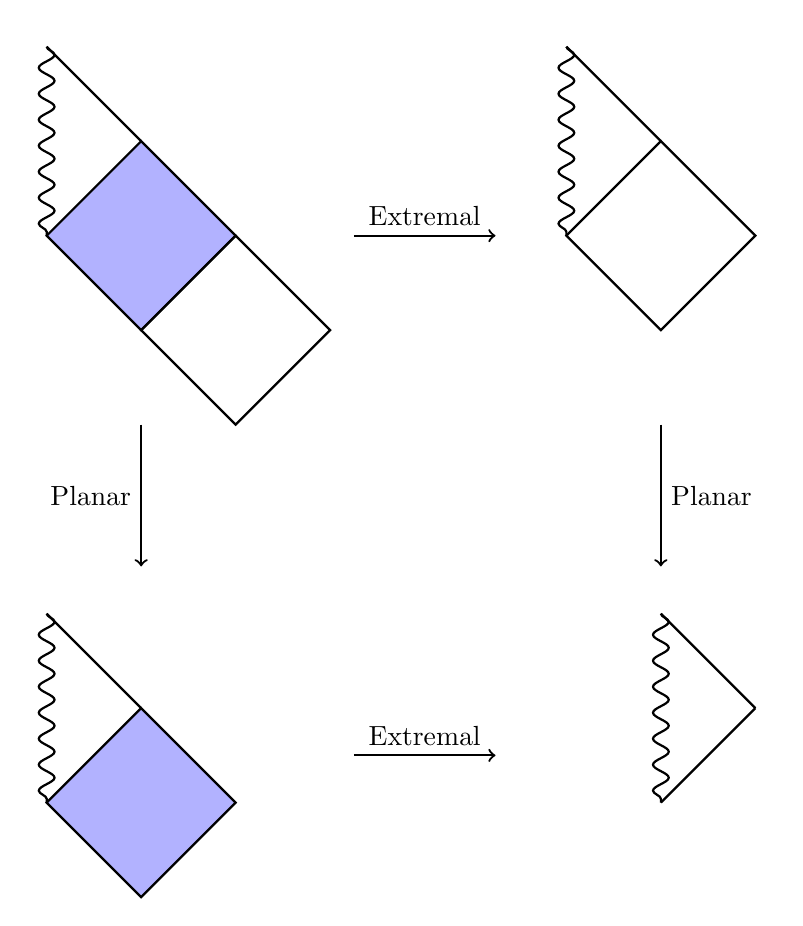
\begin{tikzpicture}[scale = 0.3]
\node (topLeft2) at (0,4) {};
\node (topLeft1) at (-4,8) {};
\node (topLeft3) at (-8,12) {};


\node (topRight1) at (18,8) {};
\node (topRight3) at (14,12) {};

\node (botLeft1) at (-4,-16) {};
\node (botLeft3) at (-8,-12) {};

\node (botRight) at (18,-12) {};


\draw[thick, ->] (5,8)-- node[midway, above] {Extremal} (11,8);
\draw[thick, ->] (5,-14)--node[midway, above] {Extremal} (11,-14);

\draw[thick, ->] (-4,0)--node[midway, left] {Planar} (-4,-6);
\draw[thick, ->] (18,0)--node[midway, right] {Planar}(18,-6);


\path
 (topLeft1) +(90:4) coordinate[label=90:] (topLeft1top)
 +(-90:4) coordinate(topLeft1bot)
 +(0:4) coordinate[label=360:] (topLeft1right)
 +(180:4) coordinate[label=180:] (topLeft1left)
 ;
\draw[thick, fill=blue!30!white]  (topLeft1left)
        -- node[midway, below, sloped] {}
         (topLeft1top)
         -- node[midway, below, sloped] {}
         (topLeft1right)
             node[midway, above, sloped] {}
           -- node[midway, above, sloped] {}
         (topLeft1bot)
         -- node[midway, above, sloped] {}
         (topLeft1left)
         -- cycle;

\path
 (topLeft2) +(90:4) coordinate[label=90:] (topLeft2top)
 +(-90:4) coordinate(topLeft2bot)
 +(0:4) coordinate[label=360:] (topLeft2right)
 +(180:4) coordinate[label=180:] (topLeft2left)
 ;
\draw[thick]  (topLeft2left)
        -- node[midway, below, sloped] {}
         (topLeft2top)
         -- node[midway, below, sloped] {}
         (topLeft2right)
             node[midway, above, sloped] {}
           -- node[midway, above, sloped] {}
         (topLeft2bot)
         -- node[midway, above, sloped] {}
         (topLeft2left)
         -- cycle;

 \path
 (topLeft3) +(90:4) coordinate[label=90:] (topLeft3top)
 +(-90:4) coordinate(topLeft3bot)
 +(0:4) coordinate[label=360:] (topLeft3right)
 ;
\draw[thick] (topLeft3top) -- (topLeft3right);
\draw[decorate,decoration={snake, segment length=3.3mm, amplitude=1mm},thick]  (topLeft3top) -- (topLeft3bot);

\path
 (topRight1) +(90:4) coordinate[label=90:] (topRight1top)
 +(-90:4) coordinate(topRight1bot)
 +(0:4) coordinate[label=360:] (topRight1right)
 +(180:4) coordinate[label=180:] (topRight1left)
 ;
\draw[thick]  (topRight1left)
        -- node[midway, below, sloped] {}
         (topRight1top)
         -- node[midway, below, sloped] {}
         (topRight1right)
             node[midway, above, sloped] {}
           -- node[midway, above, sloped] {}
         (topRight1bot)
         -- node[midway, above, sloped] {}
         (topRight1left)
         -- cycle;

 \path
 (topRight3) +(90:4) coordinate[label=90:] (topRight3top)
 +(-90:4) coordinate(topRight3bot)
 +(0:4) coordinate[label=360:] (topRight3right)
 ;
\draw[thick] (topRight3top) -- (topRight3right);
\draw[decorate,decoration={snake, segment length=3.3mm, amplitude=1mm},thick]  (topRight3top) -- (topRight3bot);

\path
 (botLeft1) +(90:4) coordinate[label=90:] (botLeft1top)
 +(-90:4) coordinate(botLeft1bot)
 +(0:4) coordinate[label=360:] (botLeft1right)
 +(180:4) coordinate[label=180:] (botLeft1left)
 ;
\draw[thick, fill=blue!30!white]  (botLeft1left)
        -- node[midway, below, sloped] {}
         (botLeft1top)
         -- node[midway, below, sloped] {}
         (botLeft1right)
             node[midway, above, sloped] {}
           -- node[midway, above, sloped] {}
         (botLeft1bot)
         -- node[midway, above, sloped] {}
         (botLeft1left)
         -- cycle;
         
 \path
 (botLeft3) +(90:4) coordinate[label=90:] (botLeft3top)
 +(-90:4) coordinate(botLeft3bot)
 +(0:4) coordinate[label=360:] (botLeft3right)
 ;
\draw[thick] (botLeft3top) -- (botLeft3right);
\draw[decorate,decoration={snake, segment length=3.3mm, amplitude=1mm},thick]  (botLeft3top) -- (botLeft3bot);

\path
 (botRight)
 +(+90:4) coordinate[label=360:] (botRighttop)
 +(-90:4) coordinate(botRightbot)
 +(0:4) coordinate[label=180:] (botRightright)
 ;

 \draw[decorate,decoration={snake, segment length=3.3mm, amplitude=1mm},thick] (botRighttop) -- (botRightbot);
 \draw[thick] (botRighttop) -- (botRightright);
  \draw[thick] (botRightbot) -- (botRightright);

\end{tikzpicture}
\caption[Comparison of the conformal diagrams for spherical and planar Reissner-Nordstr\"om-like spacetimes]{Comparison of the conformal diagrams for spherical and planar Reissner-Nordstr\"om-like spacetimes. We only display one copy of each type of region. Shaded regions are where the spacetime is dynamical (no timelike Killing vector).}
\label{fig:planarextremal}
\end{figure}


We start with the spherically symmetric extremal Reissner Nordstr\"om solution, whose causal structure we have seen is shared by a large class of BPS solutions obtained by compactifying brane configurations. Its maximal analytical extension is a sequence of two types of regions, both static: one containing an asymptotically flat exterior, the other (the interior) containing a timelike singularity which is repulsive to massive neutral particles. In other words, timelike geodesics are infinitely extendable. For our purposes, we focus on just a single pair of such regions, see Figure \ref{fig:planarextremal} for an illustration. If the solution is made non-extremal, a third type of region occurs, which is dynamical (non-stationary) and located between the two distinct static patches. Let us now consider the effect of replacing spherical by planar symmetry, or, in brane language, of delocalisation of the constituent branes along two non-compact spatial directions. In this case, the solution cannot be asymptotically flat any more. For brane-type solutions, it is a well-known feature that asymptotic flatness requires more than two transverse dimensions: `large branes' (those with two or less transverse dimensions, like the D7-brane in type IIB) cannot be asymptotically flat. In terms of the causal structure, we lose the static, asymptotically flat patch and remain with a static patch containing the singularity, and a dynamical patch. More precisely, by maximal analytic extension, we end up with two patches of each type, resulting in a conformal diagram which is the same as Schwarzschild rotated by 90 degrees, see Figure (\ref{fig:PC}). If we now perform an extremal limit, we also lose the dynamical patch and remain with a static patch containing a singularity. Comparing the four types of conformal diagrams, we see that going from spherical to planar symmetry removes the asymptotically flat region, while the existence of a dynamical patch depends on non-extremality. Viewed from this perspective, the presence of a cosmological patch in our solutions is completely natural, and results from physics already present in Einstein-Maxwell theory. These features are robust under dimensional lifting and persist for the three-charged solution, which is a solution of gauged supergravity and has the same conformal diagram \cite{Gutowski:2019iyo}. However, the Nernst brane solutions \cite{Dempster:2015,Dempster:2016,Barisch:2011ui,Cardoso:2015wcf} illustrate that these features do not persist if we modify essential features. Like the three- and four-charge solutions, the single-charged Nernst branes are planar and not asymptotically flat, but they do not share the `inside-out' feature of a singularity at a finite distance inside the static patch. The essential difference is that Nernst branes require a non-constant scalar fields, and therefore there is no limit in which they become solutions of four-dimensional Einstein-Maxwell theory. Instead, as shown in \cite{Dempster:2016}, they lift to boosted AdS-Schwarzschild black brane solutions of five-dimensional AdS gravity.

The close relation of our cosmological solutions to the planar Reissner-Nordstr\"om solution also settles the question of whether we need to interpret it as being sourced by negative tension branes. We have found that the local Komar mass is negative in the static patch, which is consistent with the repulsive character of the singularity. However, this feature is also present in the spherical Reissner-Nordstr\"om solution, the only difference being that with planar symmetry we lose the asymptotically flat region, and hence the ability to define a `proper' mass by evaluating the Komar expression at asymptotic infinity. This reflects the general insight, reviewed recently in \cite{Deser:2019acl}, that the definition of global quantities through conservation laws \emph{\`a la} Noether requires that general diffeomorphism invariance is `broken naturally' by the presence of extra structure, such as boundary conditions. That we do not have a static asymptotic region does not provide a good reason to assign negative tension to the sources because locally, the situation is not different from Reissner-Nordstr\"om. Moreover, for the cases where we can lift to ten or eleven dimensions, the sources reveal themselves as conventional, positive tension branes.

The only caveat is that our four-dimensional solutions admit other embeddings into string theory, which might change their higher-dimensional interpretation. In particular, it can be shown that the solution found in \cite{Fre:2008zd} describes a region of our solution, although in different coordinates, where the existence of a Killing horizon is not obvious. The solution of \cite{Fre:2008zd} admits an uplift over the orientifold $K3 \times \mathbb{T}^2 / \mathbb{Z}_2$. This alternative embedding, which we have not analysed in detail in this thesis, is interesting because it starts with a compactification which has less than maximal supersymmetry. In contrast, in our uplift we have used toroidal compactifications and start with maximally supersymmetric theories in ten and eleven dimensions. Therefore reduction to a four-dimensional $\N=2$ theory requires one to truncate the field content after compactification. In \cite{Fre:2008zd} the sources are orientifolds, rather than D-branes or M-branes. Some authors \cite{Cornalba:2003kd} have argued that in string theory, orientifolds naturally give rise to cosmological solutions. This is a natural direction to perform additional research, together with the proper dimensional uplift of the three-charged solution of \cite{Gutowski:2019iyo}, which as a solution of gauged supergravity would need the mechanics of the Sherk-Schwarz reduction mentioned in passing during Section \ref{sec:kkred}, rather than the simple Kaluza-Klein reduction we have concerned ourselves with within this thesis.

One aspect which we have not investigated in this chapter is the question of whether our solutions are stable. For this we refer to the discussion in \cite{Burgess:2002vu, Burgess:2003mk} which have addressed some aspects of the stability of the horizon. They found that the situation for the first horizon is the same as for the inner horizon of non-extremal Reissner-Nordstrom solution, while for the second horizon no indication for an instability was found. 

While our analysis disfavours interpreting the sources of our solutions as negative tension branes, it has been argued that negative branes exist in string theory \cite{Dijkgraaf:2016lym}. In \cite{Hull:1998ym} it was shown that when admitting timelike T-duality, the web of string/M-theories contains exotic theories with twisted supersymmetry and negative kinetic energy for some of the fields. Moreover, there exists at least one version of type-II string theory for any possible spacetime signature.  According to \cite{Dijkgraaf:2016lym}, some of the branes of these exotic theories appear as `negative branes' when viewed from the point of view of a dual theory. This could allow the construction of new, genuinely stringy cosmological solutions, and our formalism could easily be tweaked to study these solutions. We will return to this discussion in the conclusions of this thesis, which with the additional context of the next chapter, offers an interesting project for further work.
